\section{Syntax | Syntactic Parsing}
\subsection*{Description}
\emph{Task} --- Assign syntactic structure to a string by breaking it down into a hierarchy of constituents that is grammatically correct (similar to dependency parsing)

{\color{lightgray}\hrule height 0.001mm}

\emph{Terminology} ---
\begin{itemize}
    \item \emph{Constituent}: Sequence of words that function as a coherent unit resp. nodes in tree
    \begin{itemize}
        \item \emph{Terminals}: Words 
        \item \emph{Non-terminals}: Abstractions over words (e.g. NP, VP, etc.)
    \end{itemize}
    \item \emph{Grammar}: Set of production rules, according to which strings can be formed from a vocabulary
    \begin{itemize}
        \item \emph{Context-free grammar (CFG)}: Grammar where rules are applied regardless of context
    \end{itemize}
    \item \emph{Parse tree}: 
    \begin{itemize}
        \item Represents both syntactic structure of a string and its derivation under grammar
        \item Can be considered a bag of production rules and a multiset (set with repeats) since production rule can appear multiple times in the tree
    \end{itemize}
\end{itemize}

{\color{black}\hrule height 0.001mm}

\subsection*{Formulation}
\emph{Context-free grammar $(\mathcal{N}, \mathcal{S}, \Sigma, \mathcal{R})$} ---
\begin{itemize}
    \item Set of non-terminals $\mathcal{N} = \{N_1, N_2, \dots\}$
    \item Distinguished start non-terminals $\mathcal{S}$
    \item Set of terminals $\Sigma = \{a_1, a_2, \dots\}$
    \item Set of production rules $r$ of the form $N \to \alpha$, where $N$ is non-terminal (incl. $\mathcal{S}$) and $\alpha \in (\mathcal{N} \cup \Sigma)^*$, i.e. $\alpha$ is ordered sequence of terminals or non-terminals
    \item String $s$ of length $M$ 
    \item Empty string $\varepsilon$
    \item Set of all strings given by Kleene closure $\Sigma^*$
    \item $T(s)$ is set of trees $t$ that yield $s$
    \item E.g.:
    \begin{itemize}
        \item Language $\{a^i b^j c^k \mid i, j, k \geq 0, i + j = k\}$ is generated by:
        $
        \mathcal{S} \to a \mathcal{S} c \mid W$,
        $W \to bWc \mid \varepsilon
        $
        \item Language $\{a^i b^j c^k \mid i, j, k \geq 0, i + k = j\}$ is generated by:
        $
        \mathcal{S} \to KW$,
        $K \to aKb \mid \varepsilon$,
        $W \to bWc \mid \varepsilon$
        \item Language $\{w \in \{a, b\}^* \mid w \textrm{ contains min. }3 a\}$ is generated by:
        $
        \mathcal{S} \to WaW aW aW$,
        $W \to aW \mid bW \mid \varepsilon
        $
    \end{itemize}
\end{itemize}

{\color{lightgray}\hrule height 0.001mm}

\emph{Probabilistic CFGs} ---
Motivation:
\begin{itemize}
    \item Often, multiple syntactic structures are grammatically admissible, i.e. the string is ambiguous
    \item This is the case when a non-terminal can be produced by $2$ rules
\end{itemize}
Probabilistic CFGs $(\mathcal{N}, \mathcal{S}, \Sigma, \mathcal{R}, \mathcal{P})$:
\begin{itemize}
    \item Additionally define a set of probabilities $\mathcal{P}$ for each production rule
    \item Probabilities are locally normalized over each transition:
    $
    \sum_{k} p(N \to \alpha_k) = 1
    $
    where $N \to \alpha_1, \dots, N \to \alpha_k$ are expansions of node $N$
    \item E.g.
    $
    \text{NP} \to \text{VP} (p = 0.6) \mid \text{Adj} (p = 0.4)
    $
    with total $p = 1$
    \item Then, the probability of a parse tree is the multiplication of the probabilities of the rules used to create the tree:
    $
    p(t) = \prod_{r \in t} p(r) = p(S \to S_1 S_2)^{M-1} \times p(S \to X)^M \times p(X \to \sigma)^M
    $
    where:
    \begin{itemize}
        \item $p(S \to S_1 S_2)^{M-1}$: repeats the rule $S \to SS$ $M-1$ times to obtain $M$ starting nodes
        \item $X$: non-terminal
        \item $\sigma$: terminal
    \end{itemize}
    \item Probability of a string is the sum over all parse trees: $p(s) = p(S \stackrel{*}{\Rightarrow} s) = \sum_{t \in \mathcal{T}(s)} p(t)$ where $S \stackrel{*}{\Rightarrow} s$ is sequence of all production rules associated with going from start non-terminal to the string
\end{itemize}

{\color{lightgray}\hrule height 0.001mm}

\emph{Chomsky Normal Form (CNF)} ---
\begin{itemize}
    \item CFG, where production rules follow specific structure:
    \begin{itemize}
        \item $N_1 \to N_2 N_3$ are non-terminal productions
        \item $N \to a$ are terminal productions
        \item $S \to \varepsilon$ are productions generating an empty string (only if the language contains the empty string)
    \end{itemize}
    \item Prohibits cyclic rules (e.g. $N \to N$)
    \item Transform CFG to CNF:
    \begin{itemize}
        \item Remove null productions $A \to \varepsilon$ by modifying and adding replacements, e.g. if CFG contains $S \to AB | \varepsilon,\ B \to b|\varepsilon$, modify $\ B \to b$ and add $S \to A$, so that we have $S \to AB  | A | \varepsilon,\ B \to b$
        \item Remove unit productions $A \to B$ by replacing target with all its productions, e.g. if CFG contains $S \to B ,\ B \to bB|B$, replace $B$ with its productions, so that we have $S \to bB|B,\ B \to bB|B$
        \item Remove long productions $A \to B_1...B_k$ with $k > 2$ by using intermediate terminals, e.g. if CFG contains $A \to B_1B_2B_3$, add intermediate variable, so that we have $A \to B_1X_1,\ X_1 \to B_2B_3$
        \item Convert terminals in mixed rules $A \to aB$ by using intermediate terminals, e.g. if CFG contains $A \to aB$, add intermediate variable, so that we have $A \to XB,\ X \to a$
    \end{itemize}
\end{itemize}

{\color{lightgray}\hrule height 0.001mm}

\emph{Weighted CFGs} ---
\begin{itemize}
    \item A more general formulation of PCFGs
    \item Probabilities are globally normalized over all possible parse trees
    \item Probability of a parse tree:
    $
    p(t) = \frac{\prod_{r \in t} \exp(\textrm{score}(r))}{Z} = \frac{\prod_{r \in t} \exp(\textrm{score}(r))}{\sum_{t' \in T} \prod_{r' \in t'} \exp(\textrm{score}(r'))}
    $
    \item Challenge: $Z$ is infinitely large, potentially even larger than $\Sigma^*$ for ambiguous strings
    \item Initial solution: Probability of a parse tree, conditioned on string $s$:
    $
    p(t \mid s) = \frac{\prod_{r \in t} \exp(\textrm{score}(r))}{Z(s)} = \frac{\prod_{r \in t} \exp(\textrm{score}(r))}{\sum_{t' \in T(s)} \prod_{r' \in t'} \exp(\textrm{score}(r'))}
    $
    \item Challenge: $Z$ is still potentially infinitely large due to cyclic rules
    \item Final solution: Revert to CNF. Then, size of $Z$ is the number of rooted binary trees, which is the Catalan number $C_{M-1} = \frac{1}{M} \binom{2(M-1)}{M-1}$
    \begin{itemize}
        \item For $M\leq2, C_{M-1} = 1$
        \item For $M=3, C_{M-1} = 2$
        \item For $M=4, C_{M-1} = 5$
        \item $...$
    \end{itemize}
    \item With CNF, probability of a parse tree (if $s \neq \varepsilon$):
    $p(t \mid s) = \frac{\prod_{N_i \to N_j N_k, \in t} \exp(\textrm{score}(N_i \to N_j N_k)) \times \prod_{N_l \to a, \in t} \exp(\textrm{score}(N_l \to a))}{Z} = \frac{\prod_{N_i \to N_j N_k, \in t} \exp(\textrm{score}(N_i \to N_j N_k)) \times \prod_{N_l \to a, \in t} \exp(\textrm{score}(N_l \to a))}{\sum_{t' \in T(s)} \prod_{N_i \to N_j N_k, \in t'} \exp(\textrm{score}(N_i \to N_j N_k)) \times \prod_{N_l \to a, \in t'} \exp(\textrm{score}(N_l \to a))} $ where
    \begin{itemize}
        \item Non-terminal productions: $\prod_{N_i \to N_j N_k, \in t} \exp(\textrm{score}(N_i \to N_j N_k))$
        \item Terminal productions: $\prod_{N_l \to a, \in t} \exp(\textrm{score}(N_l \to a))$
    \end{itemize}
\end{itemize}

{\color{lightgray}\hrule height 0.001mm}

\emph{Span} ---
\begin{itemize}
    \item Contiguous segment of a string from word $w_i$ to $w_{j-1}$: $[i, j]$
    \item Span is \emph{admissible} if it is possible to construct a parse tree, which covers exactly that span and is a valid constituent according to the grammar, i.e. there exists a non-terminal $X$ such that $X \to w[i:j]$
    \item For string of length $M$ and parse tree that is organized hierarchically in strictly right-to-left manner (nodes expand along right diagonal of tree only), we have only one admissible span per span size:
    \begin{multicols}{2}
    \begin{itemize}
        \item $
        [M, M+1)
        $ for span size $= 1$
        \item $
        [1, M+1)
        $ for span size $= M$
        \item More generally:
        $
        [M - \textrm{span size} + 1, M + 1)
        $
    \end{itemize}
    \end{multicols}
\end{itemize}

{\color{black}\hrule height 0.001mm}

\subsection*{Optimization}
\emph{Cocke-Kasami-Younger (CKY) Algorithm} ---

\begin{itemize}
    \item Tasks:
    \begin{itemize}
        \item Compute $Z$
        \item Find best parse and its probability
        \item Solve the \emph{recognition problem}: Determine if a given string is admissible by the grammar
    \end{itemize}
    \item Requires grammar in CNF
    \item Algorithm to compute $Z$:
    \begin{itemize}
        \item Uses inside semiring or log-sum-exp semiring
        \item Chart is filled bottom-to-top, left-to-right, exhaustively combining lower-level blocks
        \item Chart entry $\textrm{Chart}[i, j, X]$ stores the probability that the non-terminal $X$ generates the substring $s_i, ..., s_j$.
    \end{itemize}
    \begin{enumerate}
        \item $M \gets |s|$ where $s$ is string\\
        $\textrm{chart} \gets \overline{0}$
        \item For $m = 1, \dots, M$:\\
        Terminal productions: For $X \to s_m$, where $s_m$ is terminal at position $m$ in string: $\textrm{Chart}[m, m+1, X] \mathrel{\oplus}= \exp(\textrm{score}(X \to s_m))$ where score is weight assigned to the given rule
        \item For span $= 2, \dots, M$:\\
        Beginning of span: For $i = 1, \dots, M-\textrm{span}+1$:\\
        End of span: $k \gets i + \textrm{span} - 1$\\
        Breaking point of span: For $j = i+1, \dots, k-1$:\\
        Non-terminal productions: For $X \to Y Z$:
        $\textrm{Chart}[i, k, X] \mathrel{\oplus}= \exp(\textrm{score}(X \to Y Z)) \otimes \textrm{Chart}[i, j, Y] \otimes \textrm{Chart}[j, k, Z]$ where
        \begin{itemize}
            \item Score is weight assigned to the given rule
            \item Chart entries contain probabilities that $Y$  resp. $Z$ generate left resp. right subtree at $i,j$ resp. $j,k$
        \end{itemize}
        \item Return $\textrm{Chart}[1, M+1, \mathcal{S}]$, which contains the normalization constant
    \end{enumerate}
    \item Complexity:
    \begin{itemize}
        \item Runtime complexity: $\mathcal{O}(M^3 |\mathcal{R}|)$
        \item Space complexity: $\mathcal{O}(M^2 |\mathcal{R}|)$
        \item For parse tree that is organized hierarchically in strictly right-to-left manner, we know $i = M - \textrm{span size} + 1$ (beginning) and $j = i+1$ (breaking point), thus, we can omit looping over $i$ and $j$
        \item Then, runtime complexity: $\mathcal{O}(M |\mathcal{R}|)$
    \end{itemize}
    \item Algorithm to find best parse and its probability: Run above algorithm with Viterbi or arctic semiring and implement backpointers
    \item Algorithm to find whether string is admissible by grammar: Run above algorithm with Boolean semiring
\end{itemize}

{\color{black}\hrule height 0.001mm}

\subsection*{Other}
\emph{Pumping lemma} ---
\begin{itemize}
    \item In any CFG, long enough strings have some kind of repeating structure
    \item Then, there exists a $k$ such that a string $s$ with $|s| > k$ can be written as $s = u x y z v$, where:
    \begin{itemize}
        \item $u, y, v$ are fixed parts, whereas $x$ and $z$ are pumpable parts
        \item $u x^n y z^n v$ is also in the CFG
        \item Not both $x$ and $z$ are not empty
        \item $|x y z| < k$
    \end{itemize}\\
    Proof:
    \begin{itemize}
        \item Consider a parse tree with height $|\mathcal{N}| + 1 = N$. This tree uses all non-terminals in $|\mathcal{N}|$. Thus, any tree with height $> N$ must include some repetition of a non-terminal symbol $A$
        \item Let $k >$ length of any string yielded by a tree with maximum height $N$
        \item If $|s| \geq k$, then $s$ must be yielded by a tree with height $> N$, meaning $s$ must include repetition of at least one non-terminal symbol $A$
        \item From this, properties follow:
        \begin{itemize}
            \item If $T$ is the entire parse tree, $T_A$ is the parse tree with root upper $A$, and $T_{AA}$ is the parse tree with root lower $A$
            \item $T_A$ has height $\leq N$, since if it were $> N$, there would need to be another recurring $A$ between $T_A$ and $T_{AA}$ which is a contradiction. Then, $|xyz| < k$, since tree with maximum height $N$ can only yield strings with length $<k$
            \item If both $x$ and $z$ were empty (i.e. we replaced $T_A$ with $T_{AA}$), we would have a tree with height $\leq N$ that yields $s$ with length $> k$, which is a contradiction. Then, $x$ and $z$ cannot be empty
            \item We can extend the proof to any $N$
        \end{itemize}
    \end{itemize}
    \item Pumping lemma shows that languages that require strict equality between counts symbols cannot be generated by a CFG: String $a^k b^k c^k = u x y z v$ must fulfill $| x y z | \leq k$. Then, if $a$ is in the string, the string cannot contain a $c$, and vice versa. Then, the string does not fulfill the requirement of strict equality of counts between symbols
\end{itemize}

{\color{lightgray}\hrule height 0.001mm}

\emph{Encoding a CRF for POS tagging as CFG} ---
\begin{itemize}
    \item E.g., given CGF:
    \begin{itemize}
        \item Start symbol expands to arbitrary non-terminals: $S \to AS \mid BS$
        \item Start symbol can also directly expand to terminals: $S \to a \mid b$
        \item Non-terminal $A$ maps to terminal $a$: $A \to a$
        \item Non-terminal $B$ maps to terminal $b$: $B \to b$
    \end{itemize}
    \item Transform grammar to encode CRF for POS tagging:
    \begin{itemize}
        \item Start of sequence transition: Start symbol expands to non-terminals for each POS tag: $S \to B_{t_1} \mid B_{t_2} \mid \dots \mid B_{ t_{|\mathcal{T}|}}$
        \item N-gram transitions: Tag associated with $B_{t_i}$ is associated with a word via $A_{t_i}$ and followed by another tag N-gram $B_{t_j}$: $B_{t_i} \to A_{t_i} B_{t_j} \quad \forall t \in \mathcal{T}$
        \item Termination rule: For last tag in string: $B_{t_i} \to A_{t_i}, \quad \forall t \in \mathcal{T}$
        \item Emissions: Maps tags to words: $A_{t_i} \to w_n, \quad \forall t \in \mathcal{T}, \forall w_n \in \mathcal{W}$
        \item In total, $O(|T|^2 + |T||W|)$ rules, $|T|^N$ for transitions between N-grams of order N and $|T||W|$ for emissions
    \end{itemize}
    \item In CRF, probability of tree: $
    p(t_1, \dots, t_N \mid s_1, \dots, s_N) \propto \prod_{n=1}^{N} \psi(t_n, t_{n-1}) \times \phi(t_n, s_n)
    $
    \item In CGF, probability of tree: $
    p(t \mid s_1, \dots, s_N) \propto \prod_{r \in t} \text{score}(r)
    $ where
    \begin{itemize}
        \item Start of sequence transition:
        $
        \text{score}(S \to B_{t_i, t_j, ...}) = \psi(\text{BOS}, t_i)
        $
        \item N-gram transitions:
        $
        \text{score}(B_{t_i} \to A_{t_i} B_{t_j}) = \psi(t_i, t_j)
        $
        \item Termination rule: 
        $
        \text{score}(B_{t_i} \to A_{t_i}) = 1
        $
        \item Emissions: 
        $
        \text{score}(A_{t_i} \to s_n) = \phi(t_i, s_n)
        $
    \end{itemize}
\end{itemize}

\begin{multicols}{2}
\textit{1) Syntactic parsing}\\
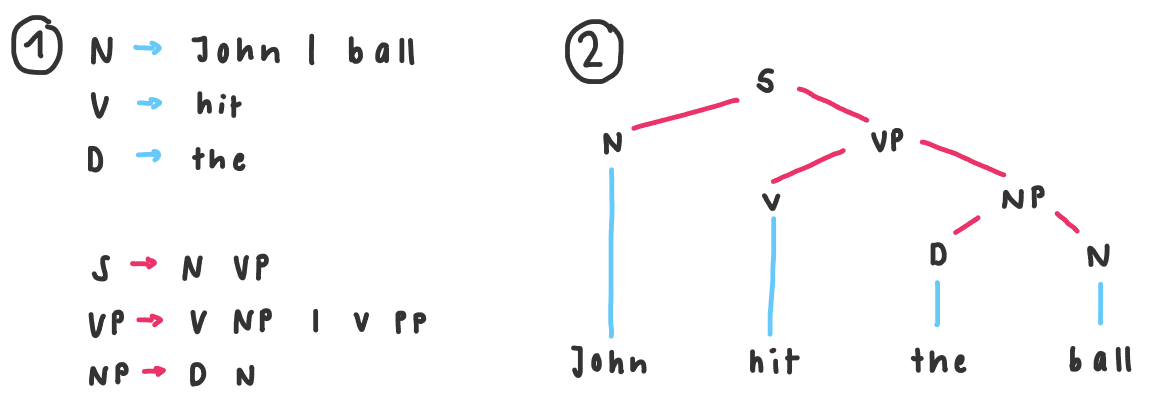
\includegraphics[height=10mm]{inhalt/images/NLP/06_syntactic_parsing_1.png}
\\\\
\textit{2) Pumping lemma}\\
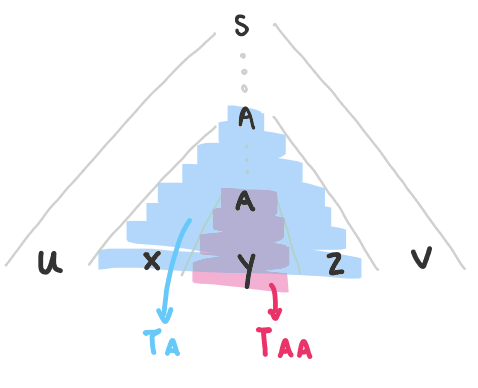
\includegraphics[height=10mm]{inhalt/images/NLP/06_syntactic_parsing_2.png}\\\\
\end{multicols}
\textit{3) CKY algorithm}\\
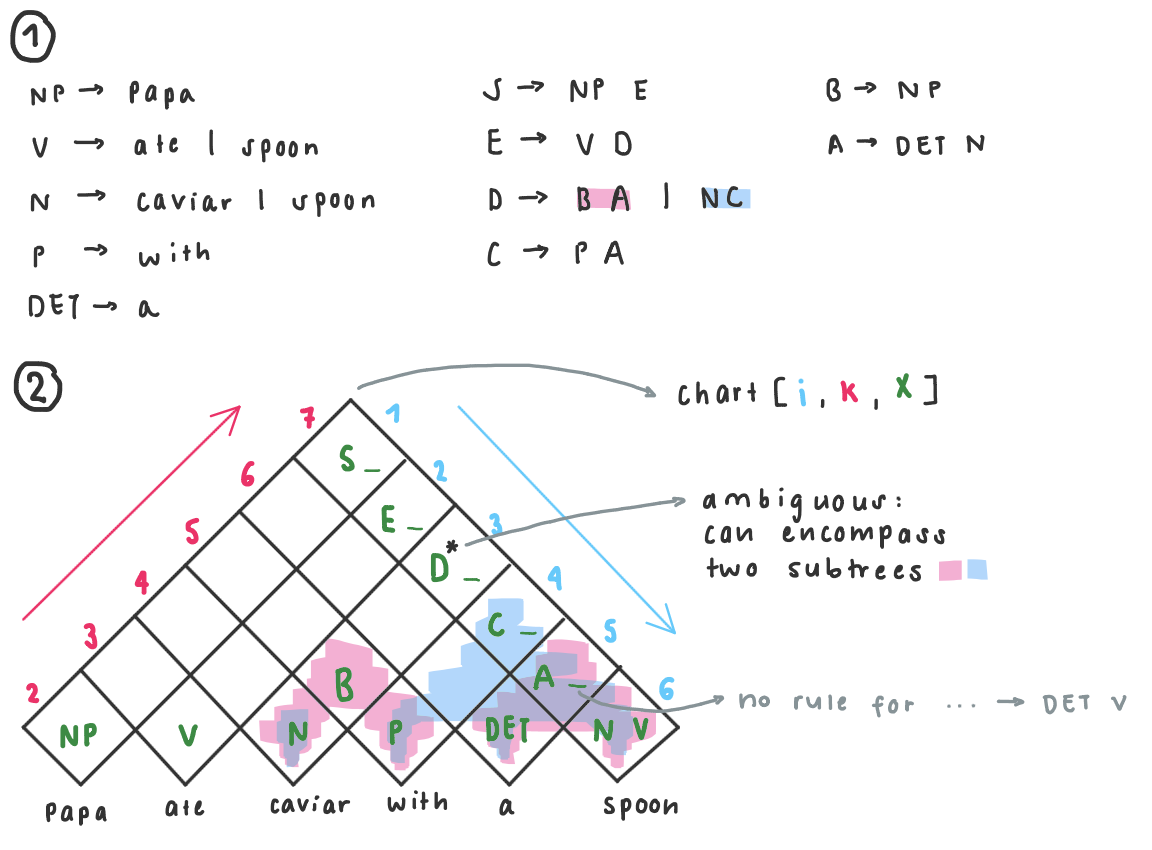
\includegraphics[height=25mm]{inhalt/images/NLP/06_syntactic_parsing_3.png}\\\\